\documentclass[12pt]{article}

\usepackage[portuguese]{babel}
\usepackage[utf8]{inputenc}
\usepackage{amsmath}
\usepackage{graphicx}
\usepackage[usenames,dvipsnames,svgnames,table]{xcolor}
\usepackage{listings}

\title{Implementação de um Ray Tracer}
\author{Miguel Correlo \\
\small{pg22780}\\
\small{correlomm@gmail.com}}
\lstdefinestyle{customc}{
  belowcaptionskip=1\baselineskip,
  breaklines=true,
  frame=L,
  xleftmargin=\parindent,
  language=C,
  showstringspaces=false,
  basicstyle=\footnotesize\ttfamily,
  keywordstyle=\bfseries\color{blue!40!black},
  commentstyle=\itshape\color{green!40!black},
  identifierstyle=\color{black},
  stringstyle=\color{orange},
}

\lstdefinestyle{customasm}{
  belowcaptionskip=1\baselineskip,
  frame=L,
  xleftmargin=\parindent,
  language=[x86masm]Assembler,
  basicstyle=\footnotesize\ttfamily,
  commentstyle=\itshape\color{green!40!black},
}

\lstset{escapechar=@,style=customc}
\begin{document}
\maketitle

\begin{abstract}
O {\it ray tracing} é uma das várias técnicas que existem para fazer {\it render} de imagens por computador. A idéia acente por trás do {\it ray tracing} é reproduzir imagens a partir da realidade física existente no mundo real. As imagens são reproduzidas a partir da luz que geralmente vem de uma fonte luminosa e é decomposta em raios. Os raios são reproduzidos por computador simulando o percurso de um determinado raio que percorre até chegar aos nossos olhos desde de um ponto de luz. Permitindo assim simular de um modo artificial o que o nossos olhos vêm.\newline

É evidente que não é tão simples quanto parece reproduzir essa realidade. É preciso de alguma forma acompanhar esses raios, o que é uma tarefa díficil pois a natureza reproduz essa realidade de um modo infinito o que leva a exigir um poder computacional que não temos à nossa disposição para a simular.\newline

Uma das ideias fundamentais do {\it ray tracing} é precisamente devido à limitação computacional só se preocupar com os raios que atingem os nossos olhos e depois com alguns dos seus ressaltos. A segunda ideia passa pela geração das imagens que são geralmente matrizes de pixeis com uma resolução limitada. As duas ideias anteriores são a base para a implementação deste {\it ray tracer}. Neste trabalho serão abordados tópicos como o lançamento dos primeiros raios, sombras, reflexões, refrações, {\it anti-aliasing, motion blur, area lights, depth of Field, path Tracing with importance sampling e finalmente russian roulette}


\end{abstract}

\section{Introdução}
\vspace{5 mm}
\hspace{8 mm} O intuito mais básico do {\it ray tracing}, na sua forma elementar, é utiliza-lo em todos sítios onde fosse necessária de alguma forma reproduzir o mundo real que nós vemos para o mundo virtual. No entanto, ainda não é possível essa flexibilidade.\newline

O {\it ray tracing} tem sido utilizado em ambiente de produção {\it off-line} durante algumas décadas até agora. O {\it rendering} de uma cena não é necessário terminar em apenas em alguns milisegundos. Porém a evolução da computação e a elaboração de novos algoritmos de renderização permitiu atingir o que agora chamamos de ``{\it ray tracing} em tempo real''. Esta evolução permitiu melhorar certos pormenores na qualidade das reflexões e muitos efeitos que até então eram muitos díficeis de alcançar, agora são bastante naturais usando um \textsl{ray tracer}. Reflexões, refrações, campos de profundidade e sombras de alta qualidade. No entanto, isto não significa que estes pormenores não exigam tempo de computação.\newline

A placa gráfica por outro lado, hoje em dia, gera a maioria das imagem mas ainda é muito limitada no \textit{ray tracing}. Mas não implica que essa limitação seja removidas no futuro. A alternativa para o \textit{ray tracing} nas placas gráficas é o uso da rasterização. A restarização é uma outra forma de abordar a geração de imagens.
A primitiva mais básica na rasterização não são os raios, mas sim os triângulos. Por cada triângulo existente na cena, estima-se a sua convertura no {\it port view} e cada píxel tocado pelo triângulo é computada a cor atual.\newline

As placas gráficas são muito boas na rasterização porque conseguem fazer muitas otimazações. Cada triângulo é desenhado independentemente do seu precedente o que é denominado por "modo imediato". No modo imediato só precisa saber que o triângulo está pronto de seguida é computada a sua cor baseada através de uma serie de atributos como variáveis globais, atributos de interpolação, textura e {\it shader programs}.\newline

Na rasterização tipicamente desenha-se as reflexões usando um passo intermediário onde se faz o render para texturas às quais alimentará para reproduzir as reflexões. No entanto, este modo tem a si associado problemas de precisão. Desta forma, entre outras otimizações permitem o desenho dos triângulo seja mais rápido.\newline

O \textit{raytracing}, por outro lado, tem que ter uma referência para toda a geometria da cena depois do raio ser lançado. De facto, não é necessário ter em conta quando se refere aos triângulos. O \textit{ray tracing} tende ser "global" e a rasterização tende a ser "local". Pois não à divergências do lado das simples decisões na rasterização, ao contrário do ray tracing.\newline

O \textit{ray tracing} não é usado sempre, uma vez que a vantagem da rápida renderização e outra técnicas como,\textit{ scan line rendering}, subdivisão de \textit{meshs} e o render rápido de \textit{micro facets}, tem ganho em relação à verdadeira soluçao de \textit{ray tracing}, especialmente no lançamento dos primeiros raios. Mas no que toca ao lançamento de raios secundários em superfícies refletidas ou refratadas todas as possibilidades estão em cima da mesa.

\section{Complicações, recursividade e o infinito}
\vspace{5 mm}
\hspace{8 mm}Os \textit{raytracers} não oferecem um solução completa, uma vez que não existem soluções completas quando estamos a lidar com o aleatório e o infinito. É muitas vezes é uma complicação dicidir o retira a uma imagem o seu realismo. Muitas das vezes, a decisão de tirar milhares de raios por píxel talvez não seja o ideal mesmo que a solução assim o pareça exigir.\newline

A iluminação global é um bom exemplo de isso mesmo. As técnicas de iluminação global como \textit{photo mapping}, tenta-se diminuir o caminho entre a luz e a superficie em que estamos. No entando na sua generalidade, para fazer uma boa iluminação global exigiria lançar uma quantidade infinita de raios em todas as direções e ver qual a percentagem desses raios atingiram a luz. Isto pode ser feito mas vai-se refletir na performa-se do algoritmo. Em vez disso, podemos é fazer o contrário, pegando na mesma ideia, mas em sentido inverso, do ponto de vista da luz e ver os raios que atingiram as superficies. Primeiro usamos essa informação para computar a luz na sua aproximação para cada ponto da superfície. Após esta primeira aproximação só seguimos o raio ou lançamos uma nova quantidade de raios se precisarmos de reproduzir uma reflexão ou refração (para uma reflexão perfeita só é necessário um raio). No entanto, a reprodução de refleções e refrações pode ter um custo muito elevado o que nos leva a decidir por um limite máximo de {\it depth recursion}.

\section{Primeiros raios}
\vspace{5 mm}
\hspace{8 mm}A primeira parte do desenvolvimento deste ray tracer vai fundamentemente basear-se no lançamento dos primeiros raios de colisão com os diferentes objetos da cena. Foram criadas as primeiras classes para os objetos plano, esfera e triângulo. Onde a partir do triângulo então poderá-se construir outros objetos mais complexos. Nesta fase foi também desenvolvida uma class Raio. Uma class auxiliar \textit{Vector} também foi escrita com papel fundamente na altura de fazer os cálculos adjacentes a vetores.
Aqui foi preparada toda a estrutura para se poder desenhar uma cena no ecrã. \newline

Primeiro para começar irá ser apresentado um pseudo-código da funcionalidade mais básica desta fase:\newline

\begin{lstlisting}
for cada pixel of the screen
{
  Final color = 0;
  Ray = { starting point, direction };
  for each object in the scene
  {
    determine closest ray object/intersection;
  }
  if intersection exists
  {
    color = getColorAt(intersectionPosition, intersectionRayDirection, sceneObjects,lightSources, ambientLight);
  }
  drawPixel(color, pixelPosition)
}
\end{lstlisting}

Agora aqui o código original, embora seja um pouco mais complexo vai ao encontro do principio básico do pseudo-código acima mencionado.\newline
\begin{lstlisting}
  for (int x = 0; x < width; x++){
    for (int y = 0; y < height; y++){
      thisone = y * width + x;

      Vector cameraRayOrigin = scaneCam.getCameraPosition();
      Vector cameraRayDirection = camDir.add(camRight.mult(xamnt - 0.5).add(camDown.mult(yamnt- 0.5))).normalize();

      Ray cameraRay(cameraRayOrigin, cameraRayDirection);

      std::vector<double> intersections;
      //find instersection for each object scene
      for (int index = 0; index < sceneObjects.size(); index++){
        intersections.push_back(sceneObjects.at(index)->findIntersection(cameraRay));
      }

      int indexOfWinningObject = winningObjectIndex(intersections);

      if (indexOfWinningObject < 0.0){
        //set background balck
        pixels[thisone].r = 0.0;
        pixels[thisone].g = 0.0;
        pixels[thisone].b = 0.0;
      }
      else{
        // index corresponds to object in our scene
        if (intersections.at(indexOfWinningObject) > accuracy){
          //determine the position and direction vectors at the point of intersection
          Vector intersectionPosition = cameraRayOrigin.add(cameraRayDirection.mult(intersections.at(indexOfWinningObject)));
          Vector intersectionRayDirection = cameraRayDirection;
          Color intersectionColor = getColorAt(intersectionPosition, intersectionRayDirection, sceneObjects, indexOfWinningObject, lightSources, accuracy, ambientLight);

          pixels[thisone].r = intersectionColor.getColorRed();
          pixels[thisone].g = intersectionColor.getColorGreen();
          pixels[thisone].b = intersectionColor.getColorBlue();
        }
      }
    }
  }
\end{lstlisting}

\subsection{A interseção mais próxima}
\vspace{5 mm}
\hspace{8 mm}Um raio está definido por um ponto de início e pela sua direção normalizada onde depois é parameterizada por uma distância aritmética \textbf{t}

\begin{figure}[!h]
\centering
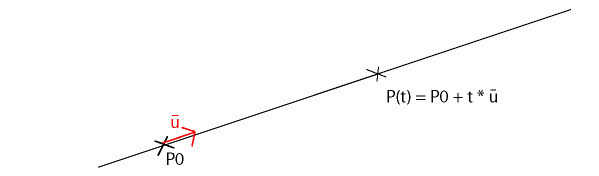
\includegraphics[scale=0.4]{img0.png}
\label{img0}
\end{figure}

O movimento é feito é feito na direção do raio desde menores distâncias, ou desde o menor \textbf{t} para o maior \textbf{t}. Vai-se percorrer cada objeto da cena e verifica-se se existe um ponto de interação, após encontrado esse ponto de interação, analisa-se qual desses pontos é o parâmetro \textbf{t} mais próximo, se for positivo significa que é em frente ao nosso ponto de partida, caso contrário fica atrás do ponto de partida.

\begin{figure}[!h]
\centering
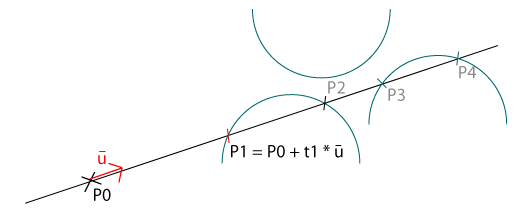
\includegraphics[scale=0.6]{img1.png}
\label{img1}
\end{figure}

\subsection{Interceção do raio com a esfera}
\vspace{5 mm}
\hspace{8 mm}


Since we're only dealing with spheres our code only contains a sphere-ray intersection function. It is one of the fastest and simplest intersection code that exists. That's why we start with spheres here. The math themselves are not that interesting we'll introduce our parameter inside an intersection equation. That will give us a second degree equation with one unknown t.

\subsection{Referências}

[1] Parallel-Split Shadow Maps for Large-scale Virtual Environments, da autoria de Fan Zhang, Hanqiu Sun, Leilei Xu, Lee Kit Lun \newline
[2] Cascaded Shadow Maps, autoria de Rouslan Dimitrov, NVidea Corporation \newline
[3] Sombras CG LEI, slides, autoria de António Ramires Fernandes \newline
[4] Notes On Implementation Of Trapezoidal Shadow Maps, autoria de Eugene K. Ressler \newline
[5] http://http.developer.nvidia.com/ \newline

\end{document}













